%%%%%%%%%%%%%%%%%%%% author.tex %%%%%%%%%%%%%%%%%%%%%%%%%%%%%%%%%%%
%
% sample root file for your "contribution" to a proceedings volume
%
% Use this file as a template for your own input.
%
%%%%%%%%%%%%%%%% Springer %%%%%%%%%%%%%%%%%%%%%%%%%%%%%%%%%%


\documentclass{svproc}
%\documentclass[graybox]{svmult}
% RECOMMENDED %%%%%%%%%%%%%%%%%%%%%%%%%%%%%%%%%%%%%%%%%%%%%%%%%%%
%

% to typeset URLs, URIs, and DOIs
\usepackage{url}
\usepackage{helvet}         % selects Helvetica as sans-serif font
\usepackage{courier}        % selects Courier as typewriter font
%\usepackage{type1cm}        % activate if the above 3 fonts are
                           % not available on your system
\usepackage{color}
\usepackage{makeidx}         % allows index generation
\usepackage{graphicx}        % standard LaTeX graphics tool
\usepackage[misc]{ifsym}                            % when including figure files
\usepackage{multicol}        % used for the two-column index
\usepackage[bottom]{footmisc}% places footnotes at page bottom
\usepackage{tabularx}
\usepackage{multirow}
\usepackage{natbib}
\usepackage{algorithm}
\usepackage{algorithmic}
\usepackage[center]{caption}
\usepackage{longtable}
\usepackage{rotating}
 \usepackage{amsmath}
\usepackage{subfigure}
\usepackage[cp1251]{inputenc}
\def\UrlFont{\rmfamily}

\begin{document}
\mainmatter              % start of a contribution
%
\title{Hamiltonian Mechanics unter besonderer Ber\"ucksichtigung der
h\"ohereren Lehranstalten}
%
\titlerunning{Hamiltonian Mechanics}  % abbreviated title (for running head)
%                                     also used for the TOC unless
%                                     \toctitle is used
%
\author{Ivar Ekeland\inst{1} \and Roger Temam\inst{2}
Jeffrey Dean \and David Grove \and Craig Chambers \and Kim~B.~Bruce \and
Elsa Bertino}
%
\authorrunning{Ivar Ekeland et al.} % abbreviated author list (for running head)
%
%%%% list of authors for the TOC (use if author list has to be modified)
\tocauthor{Ivar Ekeland, Roger Temam, Jeffrey Dean, David Grove,
Craig Chambers, Kim B. Bruce, and Elisa Bertino}
%
\institute{Princeton University, Princeton NJ 08544, USA,\\
\email{I.Ekeland@princeton.edu},\\ WWW home page:
\texttt{http://users/\homedir iekeland/web/welcome.html}
\and
Universit\'{e} de Paris-Sud,
Laboratoire d'Analyse Num\'{e}rique, B\^{a}timent 425,\\
F-91405 Orsay Cedex, France}

\maketitle              % typeset the title of the contribution

\begin{abstract}
The abstract should summarize the contents of the paper
using at least 70 and at most 150 words. It will be set in 9-point
font size and be inset 1.0 cm from the right and left margins.
There will be two blank lines before and after the Abstract. \dots
% We would like to encourage you to list your keywords within
% the abstract section using the \keywords{...} command.
\keywords{computational geometry, graph theory, Hamilton cycles}
\end{abstract}

\section{Introduction}\label{sec:intro}
The ABC simulates foraging behavior of natural honey bees for getting to the bottom of multi-dimensional and multi-model problems \cite{kumar2018artificial}. D. Karaboga in 2005 \cite{karaboga2005idea} identified that bees follow a systematic process while collecting nectar in order to produce honey. Since its inception ABC gone through numerous modifications due to its wide applicability in optimization of complex problems. The mathematical formulation of ABC algorithm in analogous to the natural behaviour of real honey bees.

The remaining article is arranged as follow: section \ref{sec:abc} explain basic ABC algorithm. Section 3 deliberates some modification in position update equation of ABC. The Arrhenius ABC algorithm is discussed in section 4. In section 5, the RPP problem explained and simulation results are discussed. Section 6 concludes this paper.

\section{Artificial Bee Colony Algorithm}\label{sec:abc}
The ABC algorithm is inspired cooperative and intelligent behavior of honey bees during the search of better quality food sources. The real honey bees lives in hive and has separation of work. These bees are cooperative with each other not competitive. Dervis Karaboga \cite{karaboga2005idea} proposed a mathematical model for working of these honey bees and divided them into two classes: employed and unemployed bees. This classification is based on task assigned to them. New food sources are identified by employed bees.
The ABC algorithm divided into three phases: employed bee phase, onlooker bee phase and scout bee phase. These phases are repeated for large number of iteration to get good solutions. These steps are discussed here.

\textbf{Initialization:} First of all, ABC initializes all the parameters and random population of bee using Eq. \ref{eq:initialization} that is analogous to solutions.

\begin{equation}\label{eq:initialization}
p_{ij}= LB_{j}+rand\times{(UB_{j}-LB_{j})}
\end{equation}

here, $i$ varies from 1 to population size and $j=1,2..,D$. Dimension of selected problem denoted by $D$. Position of $i^{th}$ solution in $j^{th}$ direction denoted by $p_{ij}$. Lower and upper bounds for search space represented by $LB_j$ and $UB_j$ accordingly. $rand$ denotes a randomly value that is selected from the range (0,1).

\textbf{Employed Bee Phase:} After initialization, next step is to select better solutions nearby the existing solutions. In this phase solution update themselves using Eq. \ref{Eq:Employed}.

\begin{equation}\label{Eq:Employed}
  V_{ij}=p_{ij}+\phi_{ij}\times(p_{ij}-p_{kj})
\end{equation}

here, $\phi_{ij} \in [-1,1]$ is an arbitrary number, $k$ varies from 1 to population size. $k$ should be different from $i$. Remaining all symbols have their usual meaning.

\textbf{Onlooker Bee Phase:} In this phase a greedy selection approach used to identify better solution for nest iteration. This selection takes place with the help of probability. The probability should be a function of fitness for each solution and computed by using Eq. \ref{Eq:prob}.
%\begin{equation}\label{Eq:fitness}
%  Fitness_{i}=
%\end{equation}
\begin{equation}\label{Eq:prob}
  Prob_{i}=\frac{fitness_{i}}{\sum_{i=1}^{colonysize/2}Fitness_{i}}
\end{equation}

\textbf{Scout Bee Phase:} If a solution is not able to update itself for long time (limit should be pre defined), then it is re-initialised using \ref{eq:initialization}.

\section{Recent Development in ABC Algorithm}\label{sec:modifications}
Initially ABC algorithm was developed and implemented for numerical optimization problems only. But now it is very popular for complex optimization problem with different characteristics. It is very simple and easy to implement. The performance of ABC algorithm mainly depends on position update equation (\ref{Eq:Employed}).

\begin{equation}\label{Eq:obl}
  ox_{ij}=UB_j+LB_j - x_{ij}
\end{equation}

Where $i^{th}$ solution in $j^{th}$ direction is denoted by $x_{ij}$ and lower and upper bounds are denoted by LB and UB in that order.
Sharma et al. \cite{sharma2016levy} initiated the idea of Levy flight search in ABC. The new position update equation depicted in Eq. \ref{Eq:levy}.

\begin{equation}\label{Eq:levy}
  x^{'}_{bestj}(t+1)=x_{bestj}(t)+step_{size}(t) \times U(0,1)
\end{equation}

Where $step_{size}$ computed using Eq. \ref{Eq:step}.
\begin{equation}\label{Eq:step}
  step_{size}(t)= 0.001 \times s(t) \times (x_{bestj}(t)=x_{kj}(t))
\end{equation}

In Eq. \ref{Eq:step} the component $s$ decided by using Eq. \ref{Eq:s} as follow:
\begin{equation}\label{Eq:s}
  s=\frac{u}{|v|^{\frac{1}{\beta}}}
\end{equation}
Where, $u$ and $v$ are computed using normal distribution and discussed in detail in \cite{sharma2016levy}.
Zhu et al. \cite{zhu2010gbest} proposed a unique variant of ABC that is to some extent inspired from particle swarm optimization and named it as Gbest-guided ABC (GABC) algorithm. Here \cite{zhu2010gbest} a new approach suggested by Zhu et al. for position update and shown in Eq. \ref{Eq:gbest}.

\begin{equation}\label{Eq:gbest}
  v_{ij}=x_{ij}+\phi_{ij} \times (x_{ij}-x_{kj}+\psi_{ij} \times (y_j - x_{ij}))
\end{equation}

Where $\psi_{ij} \times (y_j - x_{ij})$ is newly added term that guiding solution search process towards best in current swarm. $\phi$  denotes an evenly distributed arbitrary number in interval [0, C], where C denotes some positive constant  and $y_j$  represent global best solution in current swarm. The Eq. \ref{Eq:gbest} improve global best solution in present swarm by improving exploitation process. The GABC is one of the effective modification in ABC and attracted number of researchers to work on it. Like Sharma et al. \cite{sharma2016lbest} in recent times proposed modification in GABC by taking into consideration local and global best solutions. The employed bee and onlooker bee phase customized as shown in Eq. \ref{Eq:lbest} and Eq. \ref{Eq:lgbest} correspondingly.

\begin{equation}\label{Eq:lbest}
v_{ij}=x_{ij}+\phi_{ij}(x_{ij}-x_{kj})+\psi_{ij}(x_{Lbestj}-x_{ij})
\end{equation}

\begin{equation}\label{Eq:lgbest}
v_{ij}=x_{ij}+\phi_{ij}(x_{ij}-x_{kj})+\psi_{ij}(x_{Gbestj}-x_{ij})
\end{equation}

Where, local and global best values in current population denoted by $x_{Lbestj}$ and $x_{Gbestj}$ respectively. Another variant of gbest ABC proposed by Bhambu et al. in \cite{bhambu2018modified} with two amendment in basic GABC \cite{zhu2010gbest}. Here both the employed and onlooker bee phase are modified using Eq. \ref{Eq:mgbest1} and Eq. \ref{Eq:mgbest2} likewise.

\begin{equation}\label{Eq:mgbest1}
xnew_{ij}=x_{ij}+\phi_{ij}(x_{ij}-x_{kj})+ \frac{(1-t)}{T}\times \psi_{ij}(y_j-x_{ij})
\end{equation}

\begin{equation}\label{Eq:mgbest2}
xnew_{ij}=x_{ij}+\frac{(1-t)}{T}\times \phi_{ij}(x_{ij}-x_{kj})+ \psi_{ij}(y_j-x_{ij})
\end{equation}

Where, $t$ and $T$ represent present and maximum iteration count accordingly. In Eq. \ref{Eq:mgbest1} and Eq. \ref{Eq:mgbest2} two important components are defined, first one is: $\phi_{ij}(x_{ij}-x_{kj})$ that preserve the randomness of the proposed algorithm and another is: $\psi_{ij}(y_j-x_{ij})$. The second component move the solutions in the direction of global optimum and accelerate the convergence. The weight-age of these components keep changing and depends on iteration counter to maintain balancing between exploration and exploitation.

A memetic approach incorporated in ABC to enhance the performance of ABC by Bansal et al. \cite{bansal2013memetic}. In \cite{bansal2013memetic} a complex process based on GSS strategy used to decide the value of $\phi$  in Eq. \ref{Eq:Employed}. This approach update only best solutions in current swarm as it assume that better solutions lies inn closeness of highly fitted solution. A fitness based position update method established in basic ABC by Kumar et al. \cite{kumar2014fitness} with supposition that there are more probability to find the majority feasible solution in closeness of solutions with higher fitness. In \cite{kumar2014fitness} position of employed bees updated using Eq. \ref{Eq:fpabc}.
\begin{equation}\label{Eq:fpabc}
v_{ij}=x_{ij}+ \phi_{ij}(x_{ij}-x_{kj})+ (2.0-prob_i)(x_{bestj}-x_{ij})
\end{equation}

Tiwari et al. \cite{tiwari2016weight} proposed a different position update strategy based on weightage of fitness of each individual. Apart from these strategies discussed here, a number of strategies developed and applied for complex problems very efficiently in ABC. A detailed study of ABC algorithm with step by step derivation available in \cite{kumar2018artificial}.

\section{Arrhenius ABC Algorithm}\label{sec:aabc}
Some recent studies \cite{bansal2013artificial,kumar2018artificial} pointed out that major problem with ABC is unbalanced exploration and exploitation while searching for optimal solution in the given search area. This balancing may be accomplished with appropriate step size at the same time as updating position of individuals.

\section{Robot Path Planning Problem (RPPP)}\label{sec:rppp}
The considered problem has of a robot and a $2D$ search space with some obstacles. Both the starting and target positions are pre-decided for robot. There are a number of obstacles in the given search space whose co-ordinates and radius are defined by r, x-axis, and y-axis. The robot is moving in the direction of target position along with a path and in each successive iteration it tries to improve it. In order to change its direction/rotation either in left or right some handle points are there in path. The points construct an entire path from source $S$ to target $T$ characterizes as ($S$, $n1$, $n2$, $n3$, ..., $n$, $T$). It is assumed that the robot are capable to turn in both directions (left or right) in case of clashing while moving towards target. The new position of robot at time $t+1$ decided by Eq. \ref{Eq:rppp1} and Eq. \ref{Eq:rppp2}, where ($x$, $y$) denotes its current location at time $t$, $\delta t$  denotes change in time instance, $\theta$ represents the angle of rotation and $v$ is the velocity of robot.

\begin{equation}\label{Eq:rppp1}
x^{'}=x+v \times cos(\theta \delta t)
\end{equation}

\begin{equation}\label{Eq:rppp2}
y^{'}=y+v \times sin(\theta \delta t)
\end{equation}


The Eq. \ref{Eq:rppp3} shows the distance ($d$) covered by a robot with velocity $v$ .

\begin{equation}\label{Eq:rppp3}
d=\sqrt{(x^{'}-x)^2+(y^{'}-y)^2}
\end{equation}

The overall goal of the RPPP is to diminish the travelling cost i.e. total distance covered from source to destination. In order to apply the aABC algorithm to solve this problem, a 2-D workspace of the robot's motion designed according to the initial and the target positions, number of obstacles and handles. All the required parameters (maximum iteration, population, number of runs) initialized \cite{sharma2019black}. Using aABC fitness values are computed and possible collisions are detected till the termination criteria meet. Based on the fitness a greedy selection approach used to select next position for robot and it stops when reached to the target. The simulation results of the aABC \cite{kumar2019arrhenius} and ABC \cite{karaboga2005idea} are computed and compared with  Differential Evolution (DE) \cite{storn1997differential}, and Particle Swarm Optimization (PSO) \cite{kennedy1995j} on Intel core-i5 machine in MATLAB 12.1 using Windows 7 operating system. Maximum iterations for all algorithms are taken 5000. The experiments have been carried out for four different cases, shown in Table \ref{tab:cases}:

\begin{table}
\renewcommand{\arraystretch}{1.8}
\centering
\scriptsize
\caption{Cases considered for experiment}
\begin{tabular}{ccccc}
\hline
Case	&	No. of Obstacles	&	No. of Handle Points	&	Start Point	& Target Point \\
\hline
    1 & 3 & 3 & (0,0) & (10,10) \\
    2 & 9 & 5 & (0,0) & (30,30) \\
\hline
\end{tabular}
\label{tab:cases}
\end{table}


%Case1  &   3 obstacles, 3 handle points, start point (0, 0) and target point (10, 10),
%Case2  &   9 obstacles, 5 handle points, start point (0, 0) and target point (30, 30),
%Case3  &   12 obstacles, 8 handle points, start point (0, 0) and target point (50, 50),
%Case4  &   20 obstacles, 12 handle points, start point (0, 0) and target point (100,100).

\begin{figure}[t]
    \subfigure[]{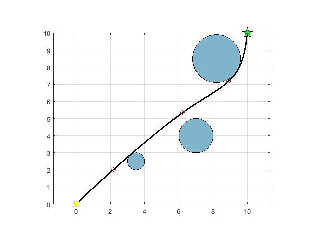
\includegraphics[width=0.23\textwidth]{Figures/Case1abc}}
    \subfigure[]{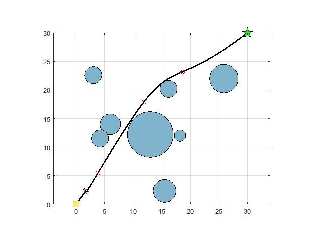
\includegraphics[width=0.23\textwidth]{Figures/Case2abc}}
    \subfigure[]{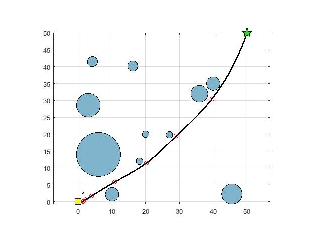
\includegraphics[width=0.23\textwidth]{Figures/Case3abc} }
    \subfigure[]{
\includegraphics[width=0.23\textwidth]{Figures/Case4abc}}
    \caption{\small{Simulation results of ABC for RPP problem}}
    \label{fig:abc}
\end{figure}



Figure \ref{fig:abc} shows the simulation result of RPP problem by using ABC, DE, PSO and aABC algorithms respectively. Numerical results are listed in Table \ref{table:results}. The Table \ref{table:results} demonstrates the outcomes of simulation for the anticipated aABC and other selected algorithms DE, ABC and PSO. The aABC is capable in finding optimal path as the optimal distance measured by the aABC is very less in contrast to the ABC, DE and PSO algorithms.

\begin{center}
\renewcommand{\arraystretch}{1.2}
\fontsize{6}{6}\selectfont
\begin{longtable}{|p{2.1cm}|p{2.1cm}|p{2.1cm}|}
\caption{Comparison of Results for the Optimal Path}\\
\hline
{Number of obstacles and handles}  &  {Algorithm} &    {Optimal Distance}   \\
\hline
\endhead
\caption{Comparison of Results for the Optimal Path}\label{table:results}\\
\hline
{Number of obstacles and handles}  &  {Algorithm} &    {Optimal Distance}   \\
  \hline
\endfirsthead
\hline
\multicolumn{2}{l}{to be cont'd on next page}
\endfoot
\endlastfoot
\multirow{4}{*}	{3 \& 3} 	&	ABC	&	14.564 \\
                            &	DE	&	14.5825  \\
                                            &	PSO	&	14.6891 \\
                                            &	aABC	&	14.5448    \\ \hline

\multirow{4}{*}	{9 \& 5} 	&	ABC	&	43.5514   \\
                                            &	DE	&	43.4917  \\
                                            &	PSO	&	45.4477 \\
                                            &	aABC	&	43.4502\\ \hline

\multirow{4}{*}	{12 \& 8} 	&	ABC	&	72.8696	\\
&	DE	&	70.7745	\\
&	PSO	&	73.0731	\\
&	aABC	&	70.4475	\\
 \hline

\multirow{4}{*}	{20 \& 12} &	ABC	&	184.0479	\\
&	DE	&	154.9557	\\
&	PSO	&	146.5722	\\
&	aABC	&	144.4057	\\
 \hline

\end{longtable}
\end{center}

\section{Conclusion}\label{sec:con}
This paper focuses on a solving robot path planning problem with a unique variant of ABC algorithm, namely Arrhenius ABC algorithm. The just anticipated aABC strategy is inspired by an exclusive concept given by Arrhenius. The exploration capability of the ABC algorithm is improved by the new method. After analysing results it can be concluded that aABC is better choice to get rid of complex optimization problems like RPPP. The results prove that aABC is best choice to solve RPP problem in comparison to other considered algorithms.

Further, the proposed method may be applied on different categories of problems. Like optimization of extracted feature set for image datasets and an attempt of improving its accuracy can be made  by incorporating some preprocessing. Also, some new strategy for path set may be implemented for RPPP.

%
% ---- Bibliography ----
%
\bibliographystyle{plain}
%\fontsize{10}{10}\selectfont
%\addcontentsline{toc}{section}{\textbf{REFERENCES}}
%\renewcommand{\bibname}{REFERENCES}
\bibliography{ref}
%\end{spacing}

\end{document}
